\documentclass[11pt,a4paper]{article}
% Main document for the final report. Compile with the companion figures,
% bibliography and measured tables supplied in this project.
\usepackage[a4paper,left=21mm,right=21mm,top=19mm,bottom=22mm,footskip=10mm]{geometry}
\usepackage[T1]{fontenc}
\usepackage[utf8]{inputenc}
\usepackage{lmodern,microtype,graphicx,booktabs,tabularx,array,enumitem}
\usepackage{amsmath,amssymb,xcolor,caption,float,fancyhdr,listings,tikz}
\usetikzlibrary{arrows.meta,positioning}
\usepackage{hyperref,xurl}
\definecolor{Ink}{HTML}{1C3543}
\definecolor{Accent}{HTML}{176764}
\definecolor{Muted}{HTML}{465C65}
\definecolor{Pale}{HTML}{F1F6F5}
\definecolor{Rule}{HTML}{B8CDCB}
\hypersetup{colorlinks=true,linkcolor=Ink,citecolor=Accent,urlcolor=Accent,
 pdftitle={Learning a balanced image distribution from biased data},
 pdfauthor={Syed Zain Afaq, Shaheer Ahmed Farooqui and Huzaifa}}
\urlstyle{same}
\setlength{\parindent}{0pt}
\setlength{\parskip}{5pt plus 1pt}
\setlength{\tabcolsep}{4pt}
\setlength{\intextsep}{8pt plus 1pt}
\renewcommand{\arraystretch}{1.15}
\clubpenalty=10000 \widowpenalty=10000 \displaywidowpenalty=10000
\hyphenpenalty=10000 \exhyphenpenalty=10000 \emergencystretch=3em
\raggedbottom
\newcolumntype{Y}{>{\raggedright\arraybackslash}X}
\newcolumntype{P}[1]{>{\raggedright\arraybackslash}p{#1}}
\makeatletter
\renewcommand\section{\@startsection{section}{1}{\z@}{2ex plus .3ex}{.7ex}{\normalfont\LARGE\bfseries\color{Ink}\raggedright}}
\renewcommand\subsection{\@startsection{subsection}{2}{\z@}{1.5ex plus .2ex}{.4ex}{\normalfont\large\bfseries\color{Accent}\raggedright}}
\newcommand{\rowsfile}[1]{\@@input generated/#1.tex }
\makeatother
\setlist[enumerate]{leftmargin=6mm,itemsep=2pt,topsep=3pt,parsep=0pt}
\captionsetup{font=small,labelfont={bf,color=Accent},justification=raggedright,singlelinecheck=false,skip=4pt}
\pagestyle{fancy}\fancyhf{}
\renewcommand{\headrulewidth}{0pt}\renewcommand{\footrulewidth}{0.4pt}
\fancyfoot[L]{\small\color{Muted}Machine Learning \enspace\textbar\enspace Final report}
\fancyfoot[R]{\small\color{Muted}\thepage}
\lstset{basicstyle=\ttfamily\footnotesize,columns=fullflexible,keepspaces=true,showstringspaces=false,breaklines=true,
 frame=single,rulecolor=\color{Rule},backgroundcolor=\color{Pale},xleftmargin=2mm,xrightmargin=2mm,framesep=4pt}
\newcommand{\Dbias}{\mathcal D_{\mathrm{bias}}}
\newcommand{\Dref}{\mathcal D_{\mathrm{ref}}}
\newcommand{\Dobs}{\mathcal D_{\mathrm{obs}}}
\newcommand{\pdata}{p_{\mathrm{data}}}
\newcommand{\pbias}{p_{\mathrm{bias}}}
\newcommand{\pobs}{p_{\mathrm{obs}}}
\newcommand{\repoURL}{\url{https://github.com/shaheer-geeksofkolachi/tiw-dsm-repro}}
\newcommand{\appURL}{\url{https://tiwdsm-cifar10-demo.streamlit.app}}
\newcommand{\weightsURL}{\url{https://github.com/shaheer-geeksofkolachi/tiw-dsm-repro/tree/main/checkpoints/deploy}}
\newcommand{\dataURL}{\url{https://github.com/shaheer-geeksofkolachi/tiw-dsm-repro/tree/main/results}}

\newcommand{\asset}[2][]{\includegraphics[#1]{figures/#2}}
\newcommand{\lead}[1]{\textbf{\color{Ink}#1}\enspace}
% auto-generated by scripts/make_report_assets.py
\def\resClfAcc{\pending}
\def\resToyref{0.483}
\def\resToyStdref{0.018}
\def\resToyobs{0.285}
\def\resToyStdobs{0.005}
\def\resToyiw{0.479}
\def\resToyStdiw{0.018}
\def\resToytiwW{0.287}
\def\resToyStdtiwW{0.007}
\def\resToytiwC{0.439}
\def\resToyStdtiwC{0.011}
\def\resToytiw{0.439}
\def\resToyStdtiw{0.006}

\begin{document}
\thispagestyle{empty}
{\sffamily\small\bfseries\color{Accent}MACHINE LEARNING \enspace\textbar\enspace FALL 2026 \enspace\textbar\enspace DELIVERABLE 3\par}
\vspace{7mm}
{\Huge\bfseries\color{Ink}Learning a balanced image distribution from biased data\par}
\vspace{2mm}
{\large\color{Muted}Reproduction and deployment of \textit{Training Unbiased Diffusion Models From Biased Dataset}, Kim and colleagues, ICLR 2024 \cite{kim2024tiwdsm}.\par}
\vspace{4mm}
{\color{Rule}\hrule}
\vspace{2mm}
\begin{tabularx}{\linewidth}{@{}P{31mm}Y@{}}
\textbf{Prepared by} & Syed Zain Afaq (36234), Shaheer Ahmed Farooqui (19722) and Huzaifa (19193)\\
\textbf{Method} & Denoising score matching with importance weights that vary with diffusion time (TIW DSM).\\
\textbf{Study setting} & Image generation on CIFAR 10. The biased sample contains 10,000 images and the reference sample contains 500.\\
\textbf{Submission} & Final report, source code and trained model. Project freeze: 25 November 2026 at 23:55.\\
\textbf{Report date} & 25 November 2026\\
\end{tabularx}
\vspace{3mm}
\subsection*{What we found}
At the same point in training, we asked two diffusion models to generate \resNimgtiw{} images each. The five classes least common in the biased data accounted for \resTailobs\% of the baseline output and \resTailtiw\% of the output from the proposed method. Their share in the target population is 50\%. The bias score also fell, from \resBiasobs{} to \resBiastiw{}. The gain in balance did not extend to overall image statistics: Fréchet Inception Distance (FID), for which lower is better, rose from \resFIDobs{} to \resFIDtiw{}, and recall fell. We therefore reproduced part of the finding of Kim and colleagues, not their improvement in FID. Each image model was trained once; both checkpoints represent 3,512,320 image exposures.
\subsection*{Code, evidence and demonstration}
\begingroup\small
\begin{tabularx}{\linewidth}{@{}P{31mm}Y@{}}
\toprule
Implementation & \repoURL\\
Trained weights & \weightsURL\quad \texttt{tiw\_dsm.pt} and \texttt{dsm\_obs.pt}\\
Recorded results & \dataURL\quad Evaluation summaries and discriminator measurements; the archive does not contain every training log.\\
Live application & \appURL\quad Streamlit Community Cloud, running on a CPU.\\
Local demonstration & \texttt{python -m streamlit run app/streamlit\_app.py}\\
Reproduction & Appendix~\ref{app:commands} gives the exact checkpoint paths. The repository guide and Kaggle notebook provide the general workflow.\\
Report source & \texttt{main.tex}, \texttt{references.bib}, \texttt{generated/} and \texttt{figures/} accompany this document.\\
\bottomrule
\end{tabularx}
\endgroup
\clearpage
\setcounter{tocdepth}{1}
\begingroup
\makeatletter
\renewcommand*\l@section[2]{\addvspace{2.5pt}\@dottedtocline{1}{0pt}{1.9em}{\bfseries #1}{#2}}
\makeatother
\tableofcontents
\endgroup
\vspace{6mm}
\begin{minipage}[t]{0.49\linewidth}\small
\listoffigures
\end{minipage}\hfill
\begin{minipage}[t]{0.47\linewidth}\small
\listoftables
\end{minipage}
\clearpage

\section{Introduction and problem statement}\label{sec:intro}
A collection with 4,030 pictures of airplanes and only 40 pictures of trucks poses a particular problem for an image generator. An airplane can look convincing even if the model produces airplanes far too often. Looking at the image tells us about its appearance. Counting what the model generates tells us whether it has learned the proportions we wanted.

Kim and colleagues \cite{kim2024tiwdsm} studied this problem with two sources of images. The large collection, $\Dbias$, comes from a biased distribution, $\pbias$. The smaller collection, $\Dref$, comes from the target distribution, $\pdata$. During training, the source of each image is known. The model is not told which class the image belongs to or how the large collection is biased. Training only on the large collection risks learning the wrong proportions. Training only on the small one gives the model little variety.

Our target was the balanced training distribution of CIFAR 10 \cite{krizhevsky2009cifar}. In the biased sample, airplanes and automobiles together account for nearly two thirds of all images. The reference sample contains just 500 images, or 5\% of the size of the biased sample. Our question was whether a generator could use the variety in the larger collection while learning proportions closer to those of the smaller one.

We implemented denoising score matching (DSM) and the paper's method, which uses importance weights that vary with diffusion time (TIW DSM, or TIW below). We first checked the training objective in two dimensions. We then trained TIW and an ordinary DSM baseline on the authors' image files with a smaller network and a shorter comparison budget. In addition to measuring class balance and image statistics, we tested how the choice of numerical solver changes the speed and quality of generation. The application lets a user compare the trained models using the same starting noise or try denoising a photograph.

\section{Literature review and background}\label{sec:lit}
\subsection{What a biased collection teaches a model}
Torralba and Efros \cite{torralba2011datasetbias} showed how decisions about image collection leave recognisable differences between vision datasets. A classifier trained on one collection may struggle with another. For a generator, the consequence can be visible in the output frequencies themselves. Our biased sample has about 100 airplanes per truck; the target has equal numbers. A measure of visual realism alone cannot tell us whether the generated class proportions have moved closer to the target.

\subsection{What the denoiser learns}
A diffusion model learns to remove Gaussian noise at a range of strengths \cite{ho2020ddpm,song2021sde}. The \emph{score} is the direction in which the logarithm of the probability density increases most rapidly at a noisy image $\mathbf{x}_t$. The true score is unknown. During training, however, we know how a clean image $\mathbf{x}_0$ was corrupted. Vincent \cite{vincent2011dsm} showed why matching this known conditional score gives the same optimum in expectation:
\begin{equation}
\mathcal L_{\mathrm{DSM}}(\theta;p)=
\tfrac12\int_0^T\lambda(t)\,
\mathbb E_{p(\mathbf{x}_0)}\mathbb E_{p(\mathbf{x}_t|\mathbf{x}_0)}
\big\|\mathbf s_\theta(\mathbf{x}_t,t)-\nabla\log p(\mathbf{x}_t|\mathbf{x}_0)\big\|_2^2\,dt .
\end{equation}
The distribution $p$ in this expression matters: training with biased images learns their score. Both implementations use the diffusion formulation of Karras and colleagues (EDM) \cite{karras2022edm}. It represents the score through a denoiser, $\mathbf s_\theta=(D_\theta-\mathbf x)/\sigma^2$, scales the network input and output according to the noise level, draws training noise strengths from a lognormal distribution and can generate images with the second order Heun solver.

\subsection{Three alternatives and their limitations}
\lead{Train on the reference set: DSM(ref).} The source distribution is right, but 500 images contain few examples of each class. A model can memorise them and generate too little variety. Augmentation helps when data are scarce \cite{karras2020ada}, but it does not supply independent examples of the target population.

\lead{Train on both sources: DSM(obs).} Including the biased images gives the model more examples. Ordinary DSM then learns the observed mixture, $\pobs$, rather than the desired distribution. In our implementation, each source supplies half the training entries. Equal representation of the two sources is not the same as equal representation of the ten classes.

\lead{Weight clean images by their importance: IW DSM.} A biased example with density ratio $w(\mathbf x)=\pdata(\mathbf x)/\pbias(\mathbf x)$ represents more target examples when this ratio is large. Choi and colleagues \cite{choi2020fair} estimated that ratio by training a classifier to distinguish the two sources. Given equally likely sources and an optimal probability $d$ of belonging to the reference source, the ratio is $d/(1-d)$. Using an estimate of this clean image ratio gives the importance weighted DSM baseline.

\subsection{Why estimate the ratio after adding noise?}
A classifier estimates density ratios reliably only if its probabilities are informative in regions shared by both distributions \cite{sugiyama2012dre}. Where the sources are easy to distinguish, a nearly certain prediction can be useful for classification but a poor estimate of the odds. Rhodes and colleagues \cite{rhodes2020tre} described this difficulty as a density chasm and used intermediate distributions to bridge it. Diffusion already provides a sequence of intermediate distributions: as noise increases, differences between the sources become less pronounced.

Kim and colleagues estimated the ratio at each noise level and used both its value and its gradient during training. Their discriminator builds on the design used for discriminator guidance \cite{kim2023dg} and a pretrained ADM image encoder \cite{dhariwal2021adm}. In their experiment in two dimensions, the integrated error of the ratio estimated across noise levels was 39.1\% of the error from an estimate that ignored time. Their image results give a separate benchmark. Our project addresses only the first column of Table~\ref{tab:paperfid}.
\begin{table}[H]\centering
\caption[Published image results]{FID reported by Kim and colleagues for the long tailed CIFAR 10 dataset, using 50,000 generated images \cite{kim2024tiwdsm}. Columns give the size of the reference set relative to the biased set. Lower values are better.}\label{tab:paperfid}
\small\begin{tabular}{lrrrr}\toprule
Method & 5\% & 10\% & 25\% & 50\%\\\midrule
DSM(ref) & 16.47 & 11.56 & 10.77 & 5.19\\
DSM(obs) & 12.99 & 10.75 & 8.45 & 7.35\\
IW DSM & 15.79 & 11.45 & 8.19 & 4.28\\
TIW DSM & \textbf{11.51} & 8.08 & 5.59 & 4.06\\\bottomrule
\end{tabular}
\end{table}


\section{Methodology of the selected paper}\label{sec:method}
\subsection{Learning to distinguish the two sources}
Both sources undergo the same Gaussian corruption. Their noisy distributions, $\pbias^t$ and $\pdata^t$, overlap more as the noise level rises and approach the same Gaussian limit. This makes estimating their ratio easier in principle. It does not ensure that a trained classifier returns accurate probabilities.

At each sampled diffusion time $t$, the discriminator $d_\phi(\mathbf x_t,t)$ receives equal numbers of noisy images from each source. Its task is to distinguish a reference image (label 1) from a biased image (label 0). These are source labels, not object classes. The discriminator minimises binary cross entropy:
\begin{equation}
\mathcal L_{\mathrm{disc}}(\phi)=-\mathbb E_t\!
\left[\mathbb E_{\pdata^t}\log d_\phi(\mathbf x_t,t)+
\mathbb E_{\pbias^t}\log\big(1-d_\phi(\mathbf x_t,t)\big)\right].
\end{equation}
With equal source probabilities, the optimum is
$d^*=\pdata^t/(\pdata^t+\pbias^t)$. The target to biased density ratio at that noise level is therefore $w^t=d^*/(1-d^*)$.

\clearpage
\subsection{Two different jobs for the same ratio}
Equation 10 of the paper \cite{kim2024tiwdsm} uses $w^t$ to change how much each example counts and $\nabla\log w^t$ to change the target that the network learns. Written for images sampled from the biased source, the objective is
\begin{equation}\label{eq:tiw}
\begin{aligned}
\mathcal L_{\mathrm{TIW}}={}&\tfrac12\int_0^T\lambda(t)\,
\mathbb E_{\pbias(\mathbf x_0)}\mathbb E_{p(\mathbf x_t|\mathbf x_0)}
\Big[w^t(\mathbf x_t)\\[-.3ex]
&{}\cdot\big\|\mathbf s_\theta(\mathbf x_t,t)
-\nabla\log p(\mathbf x_t|\mathbf x_0)-\nabla\log w^t(\mathbf x_t)\big\|_2^2\Big]\,dt .
\end{aligned}
\end{equation}
Theorem 1 in the paper states that, with the \emph{exact} ratio, this objective equals score matching on $\pdata$ up to a constant that does not depend on $\theta$. There are two reasons. First, $w^t\pbias^t=\pdata^t$: weighting changes the distribution used to average the loss. Second, $\nabla\log\pdata^t=\nabla\log\pbias^t+\nabla\log w^t$: the gradient supplies the part of the target score that ordinary DSM misses. Taking the conditional expectation over the original clean image at fixed $\mathbf x_t$ gives this target score. The theorem concerns the exact ratio, not the clipped estimate from our discriminator.

\subsection{What happens if one term is removed?}\label{sec:whyboth}
Fix the noisy image $\mathbf x_t$. Every clean image that could have produced it receives the same weight $w(\mathbf x_t)$. Multiplying the conditional squared error by this number does not change its minimiser. With sufficient capacity, \emph{weighting alone} therefore still learns the biased conditional mean $\mathbb E[\nabla\log p(\mathbf x_t|\mathbf x_0)\mid\mathbf x_t]=\nabla\log\pbias^t$. It can change the relative training effort and the variation in gradients across noisy images.

With the exact ratio, \emph{correction alone} targets the desired score, but the frequency with which regions contribute to training still follows the biased data. Using both terms changes the target and the relative contribution of each region. The authors tested these alternatives at the 5\% setting. FID was 12.99 without either term, 13.27 with weighting alone, 11.62 with correction alone and 11.51 with both \cite{kim2024tiwdsm}. Section~\ref{sec:verify} describes our smaller test of the same distinction.

\subsection{The objective used in our implementation}\label{sec:practical}
Our denoiser trains on both sources. Repeating each reference image 20 times gives an equal mixture, $\pobs=\tfrac12\pbias+\tfrac12\pdata$. The denominator of the required ratio is now the \emph{mixture}, not the biased source. Equation 36 of the paper gives
\begin{equation}
\tilde w^t=\frac{\pdata^t}{\pobs^t}
=\frac{2w^t}{1+w^t}=2d^*, \qquad
\nabla\log\tilde w^t=\nabla\log d^* .
\end{equation}
This is why the implementation uses $2d$ rather than the odds $d/(1-d)$ when training the generator. The weight lies between 0 and 2. A bounded weight is useful, but is not enough to ensure stable training or an unbiased result.

For a clean image $\mathbf y$, let $\mathbf x=\mathbf y+\sigma\mathbf n$ with standard Gaussian noise $\mathbf n$. The conditional score is $(\mathbf y-\mathbf x)/\sigma^2$ and the EDM model predicts $(D_\theta-\mathbf x)/\sigma^2$. Substitution into Equation~\ref{eq:tiw}, now using the mixture ratio, gives the following denoiser expression:
\begin{equation}\label{eq:edmtiw}
\frac{\tilde w}{\sigma^4}
\left\|D_\theta(\mathbf x;\sigma)-
\left(\mathbf y+\sigma^2\nabla_{\mathbf x}\log d_\phi(\mathbf x,\sigma)\right)\right\|_2^2 .
\end{equation}
The usual clean target $\mathbf y$ has become $\mathbf y+\sigma^2\nabla_{\mathbf x}\log d_\phi$. We retain the EDM noise weighting $\lambda(\sigma)=(\sigma^2+\sigma_d^2)/(\sigma\sigma_d)^2$; the theoretical objective allows a choice of time weighting. The discriminator expects variance preserving (VP) coordinates. We set $\alpha=1/\sqrt{1+\sigma^2}$, pass it $\alpha\mathbf x$, and choose VP time $\tau$ so that $\alpha(\tau)=\alpha$. Differentiating with respect to the original $\mathbf x$ includes the factor $\alpha$ from the chain rule.

\lead{Numerical safeguards.} We used $\bar d=\mathrm{clip}(d_\phi,10^{-5},1-10^{-5})$ before taking the logarithm. The weight is $2\bar d$; the correction uses $\nabla_{\mathbf x}\log\bar d$. Both are detached before the generator update. Outside the clipping interval, the derivative through the clamp is zero. A very small raw probability therefore does not imply a large correction in our code. We also apply \texttt{torch.nan\_to\_num} to the input gradient, handle nonfinite generator gradients before the optimiser step and use automatic mixed precision. We did not run separate experiments to measure the effects of these choices.

\begin{figure}[H]\centering
\fcolorbox{Rule}{Pale}{\begin{minipage}{0.94\linewidth}\small
\lead{First, train the discriminator head.}
\begin{enumerate}
\item For each of 10,000 updates, draw 128 images from each source. Assign labels 1 and 0 to the reference and biased images respectively. Draw VP times by importance sampling and draw Gaussian noise $\mathbf z$.
\item Form $\mathbf x_\tau=\alpha(\tau)\mathbf x_0+\sqrt{1-\alpha(\tau)^2}\,\mathbf z$. Use binary cross entropy to update the head. The pretrained ADM feature extractor remains fixed.
\end{enumerate}
\lead{Next, fix the discriminator and train the denoiser.}
\begin{enumerate}
\item Sample $\mathbf y$ from $\Dobs$, apply a random horizontal flip, and sample $\ln\sigma\sim\mathcal N(-1.2,1.2^2)$. Form $\mathbf x=\mathbf y+\sigma\mathbf n$.
\item Evaluate the clipped $d$ at $(\alpha\mathbf x,\tau(\sigma))$. Compute $\mathbf g=\mathrm{nan\_to\_num}(\nabla_{\mathbf x}\log d)$ and detach both $d$ and $\mathbf g$.
\item Minimise $\lambda(\sigma)\,2d\,\|D_\theta(\mathbf x;\sigma)-(\mathbf y+\sigma^2\mathbf g)\|^2$, averaging over examples and pixels. Scale the loss for backpropagation, check the gradients and update the denoiser with Adam. Maintain an exponential moving average (EMA) of its weights.
\end{enumerate}
\end{minipage}}
\caption[Training procedure]{The discriminator supplies a training signal. Generating an image later requires only the trained denoiser and a sampler.}\label{alg:tiw}
\end{figure}

\section{Implementation and attribution}\label{sec:impl}
\subsection{Organisation of the code}
We kept data preparation, training and evaluation separate so that a fault in one stage could be tested without repeating the rest. The library is in \texttt{tiwdsm/}; the scripts call the library.
\begin{center}\small
\begin{tabularx}{\linewidth}{@{}P{43mm}Y@{}}\toprule
Location & Responsibility\\\midrule
\texttt{tiwdsm/data.py} & Read the authors' arrays, assemble the observed mixture, scale pixels and apply horizontal flips.\\
\texttt{tiwdsm/unet.py} & Define the denoising network and its \texttt{tiny}, \texttt{small} and \texttt{base} sizes.\\
\texttt{tiwdsm/edm.py} & Set EDM scaling, draw noise strengths, weight the loss, sample with Heun or Euler and maintain EMA weights.\\
\texttt{tiwdsm/vpsde.py} & Convert EDM noise strengths to VP time and sample times by importance.\\
\texttt{tiwdsm/discriminator.py} & Estimate the source probability, the mixture weight $2d$, the gradient $\nabla\log d$ and the clean image weight for IW.\\
\texttt{tiwdsm/losses.py} & Implement DSM on either dataset, IW, TIW and the variants that omit weighting or correction.\\
\texttt{tiwdsm/metrics.py} & Compute FID, precision, recall, bias and the share of each class.\\
\texttt{scripts/} & Prepare data, train the discriminator and denoiser, evaluate models, run the sampling and toy experiments and produce report figures.\\
\texttt{app/streamlit\_app.py} & Load the deployment weights and run the interactive demonstration.\\\bottomrule
\end{tabularx}\end{center}

\subsection{Denoiser and discriminator}
We wrote a compact U shaped network following the DDPM++ design. Residual blocks use group normalisation and SiLU activations. A two layer perceptron maps a positional encoding of $c_{\rm noise}=\tfrac14\ln\sigma$ to an additive noise embedding. The network uses attention at $16\times16$ resolution and at the bottleneck, scales skip connections by $\sqrt{1/2}$, initialises the output layers to zero and uses a dropout rate of 0.13. The \texttt{small} model has 64 base channels, channel multipliers $(1,2,2,2)$ and two blocks per level, for a total of 8,952,067 parameters. The paper used approximately 56 million. Our \texttt{base} preset has 53.6 million, but we did not train it or treat it as an exact copy of the larger architecture.

For the discriminator we used the authors' pretrained ADM encoder, \texttt{32x32\_classifier.pt}. Its 47.8~million fixed parameters map a noisy image to an $8\times8\times512$ feature array. A second encoder with depth 2, width 128 and attention pooling maps these features to one source logit. Only its 2.9 million parameters are trained. Embeddings supply VP time. We also implemented a small convolutional network as an alternative feature extractor; none of the reported image results use it.

\subsection{Training settings and computing environment}
A training exposure counts one presentation of one image, including repeats. Unless otherwise stated, our image comparison uses the checkpoint at 3,512,320 exposures for \emph{each} model. Table~\ref{tab:config} separates this comparison point from the actual end of each run.
\begin{table}[H]\centering
\caption[Training settings]{Settings reported in the paper or its official training command, compared with our image experiments. Differences listed here were not varied one at a time.}\label{tab:config}
\small\begin{tabularx}{\linewidth}{@{}P{28mm}P{44mm}Y@{}}\toprule
Setting & Original configuration & Our configuration and its significance\\\midrule
Hardware & Four RTX 4090 graphics processors & Two Kaggle Tesla T4 processors. We trained one model on each; the session limit restricted the exposure budget.\\
Denoiser & DDPM++, about 56 million parameters & DDPM++ design, \resParams{} million parameters. Both models had less capacity than the original.\\
Batch and learning rate & 256 images, peak $10^{-3}$, rising over 10 million exposures & Same rate schedule and effective batch. TIW accumulated two groups of 128 images to fit in memory.\\
Duration & 11 million exposures & DSM(obs) reached \resMimgobs{} million; TIW reached \resMimgtiw{} million. At the matched checkpoint the learning rate was about 35\% of its peak.\\
EMA and dropout & Half life of 0.5 million exposures; dropout 0.13 & Both unchanged.\\
Augmentation & EDM augmentation with probability 0.12 & Horizontal flips only, giving less regularisation on the 10,380 distinct images.\\
Arithmetic & 32 bit floating point & 16 bit autocasting, loss scaling and safeguards for nonfinite gradients. The effect on quality was not isolated.\\
Discriminator & ADM features and trained head; 10,000 updates of 128 images per source & Same design and batch. Learning rate $3\times10^{-4}$ from the official script; training took \resDiscMinutes{} minutes on a T4.\\
Score correction & $\nabla\log\tilde w$ & Gradient of the clipped $\log\bar d$ with the safeguards in Section~\ref{sec:practical}.\\
FID evaluation & EDM evaluator, 50,000 generated images against the CIFAR training set & \texttt{pytorch-fid}, using the same family of Inception weights and all 50,000 training images. Implementations can differ numerically.\\
Sampler & Heun, 18 steps and 35 network evaluations & Same in the main comparison.\\
Bias classifier & VGG13 with batch normalisation & Same architecture family \cite{chenyaofo2021cifar}, \resClfAcc\% test accuracy. We did not establish that the weights are identical.\\\bottomrule
\end{tabularx}
\end{table}
The software targets Python 3.10 or later and PyTorch 2.1 or later \cite{paszke2019pytorch}. Training used CUDA on two T4 processors with 15 GB each; generation also runs on a CPU. The training session lasted about 11.3 hours; the evaluation session lasted about three hours. Dependencies include NumPy, SciPy, Pillow, PyArrow, gdown, Matplotlib, Streamlit \cite{streamlit} and version 0.3.0 of \texttt{pytorch-fid} \cite{seitzer2020pytorchfid}. The requirements specify mostly version ranges, not a record of every installed package version. Training used seed 0 for each model. Different code paths and batch accumulation mean that the same nominal seed need not give identical initial weights or training noise. At evaluation, we deliberately paired the noise seeds.

\subsection{Who contributed what}\label{sec:attrib}
\begin{table}[H]\centering
\caption[Attribution of code and results]{The components written by our group, the components adapted or reused, and the origin of the results.}\label{tab:attrib}
\small\begin{tabularx}{\linewidth}{@{}P{32mm}Y@{}}\toprule
Category & Contribution\\\midrule
Written by our team & The denoiser, source classifier interface, weight and gradient calculations, EDM forms of the losses, comparison variants, data pipeline and recovery of labels. We wrote the training loops, including resumption, time limits, EMA and mixed precision. We also wrote the evaluation routines, including a Fréchet distance calculation compatible with newer SciPy versions and precision and recall using nearest neighbours. The toy experiment, solver study, report generation and Streamlit application are ours.\\
Adapted from published work & We implemented the EDM preconditioning, noise schedule, Heun sampler and averaging rule from Karras and colleagues \cite{karras2022edm}. VP conversion and time sampling follow the authors' \texttt{classifier\_lib.vpsde}; discriminator settings follow their \texttt{train\_classifier.py} \cite{tiwdsmcode}.\\
Reused & We obtained the OpenAI ADM encoder through the official repository. In \texttt{nn.py} we bypassed legacy activation checkpointing for mixed precision; in \texttt{fp16\_util.py} we removed an unused logger import. The first edit changes memory use and recomputation, not the architecture. We reused the authors' data and pretrained encoder weights, the Inception network distributed with \texttt{pytorch-fid}, and the VGG13 classifier from Chen \cite{chenyaofo2021cifar}. We did not run the official training or sampling scripts.\\
Results & Table~\ref{tab:paperfid} and the paper column in Table~\ref{tab:main} cite the original experiments. Our other numerical results come from the recorded summaries; the text also reports rounded and derived values. Screenshots document runs of our application, not separate tests of image quality.\\\bottomrule
\end{tabularx}
\end{table}

\subsection{Checks before training on images}\label{sec:verify}
Before committing graphics processor time, we ran the scripts on a CPU using synthetic files with the same layout as the research data and a network with about 0.7 million parameters. This exercise covered data preparation, discriminator and denoiser training, resuming from a checkpoint, evaluation, the solver experiment, report generation and application startup without a browser window.

The next check used a problem in two dimensions. Two Gaussian clusters have centres $(-2,-2)$ and $(2,2)$ and identity covariance. The biased source draws 90\% of its points from the first cluster and 10\% from the second; the target draws half from each. We used 10,000 biased examples and 500 reference examples. With equal sampling from the two sources, ordinary DSM should put about $0.5(0.10)+0.5(0.50)=0.30$ of its output in the second cluster. Small perceptrons let us test the same loss, coordinate conversion and sampler as the image models against this known answer.
\begin{table}[H]\centering
\caption[Minority cluster in two dimensions]{Share of generated points in the second cluster. Values are means and standard deviations over three seeds, with 20,000 samples per seed. The target is 0.500.}\label{tab:toy}
\small\begin{tabular}{lcc}\toprule
Training method & Mean share & Standard deviation\\\midrule
DSM(ref) & \resToyref & \resToyStdref\\
DSM(obs) & \resToyobs & \resToyStdobs\\
IW DSM & \resToyiw & \resToyStdiw\\
Weighting only & \resToytiwW & \resToyStdtiwW\\
Correction only & \resToytiwC & \resToyStdtiwC\\
TIW DSM & \resToytiw & \resToyStdtiw\\\bottomrule
\end{tabular}\end{table}
\begin{figure}[H]\centering
\asset[width=\linewidth]{toy_2d.png}
\caption[Generated points in two dimensions]{Results for seed 0. Weighting alone leaves most points in the first cluster. Adding score correction moves the second cluster closer to its target share.}\label{fig:toy}
\end{figure}
The baseline gave \resToyobs{}, close to 0.30. Weighting alone gave \resToytiwW{}. Adding correction raised the share to \resToytiwC{} on its own and \resToytiw{} with weighting. Neither reached 0.50. The clean image weighting analogue and reference only training came closer in this simple setting. The test supports the \emph{direction} of our correction; it is not evidence that TIW outperforms those alternatives on images. Finite training, imperfect ratios and numerical approximations can all affect the result.


\section{Dataset, preprocessing and exploratory analysis}\label{sec:data}
\subsection{Composition and source labels}
CIFAR 10 contains colour images of ten object classes at a resolution of $32\times32$ pixels. The balanced training set contains 5,000 images per class and defines our target distribution \cite{krizhevsky2009cifar}. We used the two arrays released by the authors for their 5\% experiment. Despite the filenames, both contain real CIFAR images: \texttt{fake\_data.npz} is the biased source and \texttt{real\_data.npz} is the reference source.
\begin{table}[H]\centering
\caption[Composition of the data]{Properties of the arrays used in the experiment. The 5\% refers to 500 relative to 10,000, not to 5\% of the complete CIFAR training set.}\label{tab:dataset}
\small\begin{tabularx}{\linewidth}{@{}P{29mm}YYY@{}}\toprule
Property & Balanced target & Biased source $\Dbias$ & Reference source $\Dref$\\\midrule
Images & 50,000 & 10,000 & 500\\
Shape and type & $32\times32\times3$, uint8 & $32\times32\times3$, uint8 & $32\times32\times3$, uint8\\
Sampling & 5,000 per class & Largest class is 100.75 times the smallest & Random sample from the target population\\
Purpose & Target for FID & Main collection for training & Examples of the desired distribution\\\bottomrule
\end{tabularx}\end{table}
\begin{figure}[H]\centering
\asset[width=\linewidth]{sample_grid.png}
\caption[Raw examples by class]{One unprocessed image per class from the biased set (top) and the reference set (bottom).}\label{fig:samplegrid}
\end{figure}
Neither file contains object labels. For analysis, we matched a SHA 1 hash of each image's pixel values against the official training set. All 10,500 entries matched. The denoiser and source discriminator never received these recovered class labels. The separate classifier used for evaluation had been trained with class labels; the distinction matters when describing the supervision used by this project.

\subsection{How uneven are the two sources?}
In class order (airplane, automobile, bird, cat, deer, dog, frog, horse, ship and truck), the biased counts are 4,030, 2,416, 1,448, 868, 520, 312, 187, 112, 67 and 40. Airplanes and automobiles account for 64.46\% of the data. Ships and trucks together account for only 1.07\%. The reference counts in the same order are 51, 65, 43, 47, 50, 40, 53, 50, 45 and 56. The largest reference class is 1.625 times the smallest ($65/40$). The sample is much closer to balance, but 40 to 65 examples per class cannot describe the target exactly.
\begin{figure}[H]\centering
\asset[width=\linewidth]{class_distribution_d2.png}
\caption[Class frequencies in the two sources]{The logarithmic scale on the biased counts makes the rare classes visible. The class counts in the smaller reference sample also vary, although far less.}\label{fig:classdist}
\end{figure}

\subsection{Image quality and overlap}
We found no invalid shapes, corrupted images, missing pixel values or exact duplicates within either file. There were 120 images common to both files. We retained them because removing them would have changed the authors' split. Their score training archive has 20,000 entries but only 10,380 distinct images. We reconstructed that same collection directly from the arrays by keeping each biased entry once and repeating the reference entries 20 times.

The mean red, green and blue values in the biased set were 0.499, 0.504 and 0.492 after scaling the pixels to the interval $[0,1]$. The target means were 0.491, 0.482 and 0.447. These differences are consistent with a change in the mix of classes. Channel averages cannot rule out other kinds of bias within a class.
\begin{figure}[H]\centering
\asset[width=.87\linewidth]{channel_stats.png}
\caption[Colour statistics]{Mean and standard deviation of each colour channel on a scale from zero to one.}\label{fig:channels}
\end{figure}

\subsection{Preparing a training batch}
The images already have the resolution the network needs. The important preprocessing decisions concern the source mixture, the pixel scale and the way noise is added.
\begin{table}[H]\centering
\caption[Training pipeline]{How the raw arrays become batches for the denoiser and the discriminator.}\label{tab:prep}
\small\begin{tabularx}{\linewidth}{@{}P{33mm}Y@{}}\toprule
Stage & Operation and reason\\\midrule
Acquire and validate & Read both released archives and the official CIFAR training and test sets. Check shapes, data types, ranges and missing values. Use pixel hashes to recover analysis labels.\\
Build $\Dobs$ & Combine 10,000 biased entries with $20\times500$ reference entries. Each source supplies half of the observed distribution, which is why the mixture weight is $2d$.\\
Convert pixels & Move the colour channel from last to first, convert unsigned bytes to 32 bit floats, and apply $x/127.5-1$. The resulting range is $[-1,1]$, consistent with the EDM setting $\sigma_{\rm data}=0.5$.\\
Denoiser examples & Apply random horizontal flips for variation without changing resolution. Shuffle and train on effective batches of 256.\\
Discriminator examples & Use no flip. Apply VP perturbations at times drawn by importance sampling, as in the official discriminator script. Each batch contains 128 examples from each source.\\\bottomrule
\end{tabularx}\end{table}

\section{Reproduction results}\label{sec:results}
\subsection{What the measurements mean}
\lead{Fréchet Inception Distance (FID).} Following the original evaluation, we compared \resNimgtiw{} generated images per model with features from all 50,000 balanced training images \cite{heusel2017fid}. FID compares the means and covariances of Inception features. A smaller value indicates closer agreement, not a percentage of correct images. We used \texttt{pytorch-fid} with Inception weights ported from TensorFlow. Both models used the same noise seeds, 0 through 49,999, and the Heun solver with 18 steps. These require 35 network evaluations (NFE).

\lead{Precision and recall.} We used neighbourhoods defined by the three nearest neighbours in the feature space, with 10,000 real and 10,000 generated feature vectors \cite{kynkaanniemi2019pr}. Precision asks how much generated output lies within the region represented by real examples. Recall asks how much of the real region the generator covers. They describe image distributions, not the accuracy of an object classifier.

\lead{Bias and class shares.} Equation 51 of the paper compares the mean class probabilities assigned to the reference set and to the generated images:
\[
B=\sum_z\left|\mathbb E_{\mathbf x\sim\Dref}p(z\mid\mathbf x)-
                 \mathbb E_{\mathbf x\sim p_\theta}p(z\mid\mathbf x)\right|.
\]
The probabilities come from a pretrained VGG13 classifier with batch normalisation \cite{simonyan2015vgg,chenyaofo2021cifar}. Its CIFAR test accuracy was \resClfAcc\%. A smaller $B$ indicates closer agreement with the reference set. Separately, we counted the class with the largest predicted probability for each generated image, calculated the $L_1$ distance of that histogram from uniform, and measured the combined share of dog, frog, horse, ship and truck. These five \emph{tail classes} make up 50\% of the target population and 7.2\% of the biased sample. A correct combined share need not mean that each individual share is correct.

\subsection{Can the discriminator distinguish the sources?}
We examined 500 training images from each source. At low noise the discriminator separated the sources with about 99\% balanced accuracy. As noise rose, the two sets became harder to tell apart. By $\tau=1$ the mean predicted source probabilities were almost the same, and accuracy was \resDiscAccHigh\%. These are training measurements, not an independent calibration test.
\begin{table}[H]\centering
\caption[Discriminator by noise level]{Output of the ADM discriminator after \resDiscMinutes{} minutes of training. The last column shows the median \emph{odds} $d/(1-d)$ for biased images, not the weight $2d$ used on the mixture. Values are rounded.}\label{tab:disc}
\small\begin{tabular}{rrrrrr}\toprule
VP time $\tau$ & EDM $\sigma$ & Accuracy (\%) & Mean $d$ on $\Dref$ & Mean $d$ on $\Dbias$ & Median odds\\\midrule
\rowsfile{disc_table}
\bottomrule\end{tabular}\end{table}
\begin{figure}[H]\centering
\asset[width=.88\linewidth]{disc_diag.png}
\caption[Source separation as noise increases]{Balanced accuracy falls from \resDiscAccLow\% at $\tau=0.01$ to \resDiscAccHigh\% at $\tau=1$. High noise leaves little information about the image source.}\label{fig:disc}
\end{figure}

\subsection{What happened during training}
We trained the models in parallel on separate T4 processors. DSM(obs) completed \resMimgobs{} million exposures in \resHoursobs{} hours, or \resSecKimgobs{} seconds per 1,000 images. TIW first required \resDiscMinutes{} minutes to train its discriminator. Denoiser training then took \resHourstiw{} hours before the session limit, reaching \resMimgtiw{} million exposures at \resSecKimgtiw{} seconds per 1,000 images. TIW required a forward pass and an input gradient through the fixed feature extractor, and accumulated gradients over two groups of 128 images.

In our setting, TIW took about $8.6/2.2\approx3.9$ times as long per training image as DSM(obs). Kim and colleagues reported 0.26 and 0.34 seconds per batch on four RTX 4090 processors, but their comparison was \emph{IW DSM against TIW DSM}, not DSM(obs) against TIW. The two timing ratios do not answer the same question. Nor can the two training losses be compared by their height: TIW changes the weight and target of the loss. Its logged mixture weights had a mean of about 0.84 and a standard deviation of about 0.91. Those two summaries do not reveal the whole distribution.
\begin{figure}[H]\centering
\asset[width=\linewidth]{training_curves.png}
\caption[Training measurements]{From left to right: training loss, batch mean and standard deviation of $\tilde w=2d$, and seconds per 1,000 images. Under the ideal mixture ratio the mean weight is one.}\label{fig:curves}
\end{figure}

\subsection{Main comparison at equal training exposure}
\begin{table}[H]\centering
\caption[Main reproduction results]{Results for the 5\% reference setting. The paper FID column comes from Kim and colleagues \cite{kim2024tiwdsm}. All remaining columns contain our measurements. Blank cells have no published counterpart. The second group is a longer baseline run, and the last group contains real datasets rather than theoretical bounds.}\label{tab:main}
\footnotesize\setlength{\tabcolsep}{3.6pt}
\begin{tabular}{@{}lrrrrrrr@{}}\toprule
Model or source & Paper FID & Our FID & Precision & Recall & Bias $B$ & Tail (\%) & $L_1$\\\midrule
\rowsfile{main_rows}
\midrule
\rowsfile{real_rows}
\bottomrule\end{tabular}\end{table}
At 3,512,320 exposures per model, the bias score fell from \resBiasobs{} to \resBiastiw{}, a relative reduction of \resBiasRed\% using the unrounded measurements. The distance of the class histogram from uniform fell from \resLoneobs{} to \resLonetiw{}. The share of the five tail classes rose from \resTailobs\% to \resTailtiw\%, close to their combined target of 50\%.

Image statistics told a different story. FID increased from \resFIDobs{} to \resFIDtiw{}, whereas the paper reported a decrease from 12.99 to 11.51. TIW precision rose from \resPrecobs{} to \resPrectiw{}, but recall fell from \resRecallobs{} to \resRecalltiw{}. In feature space, a greater fraction of generated examples fell within the region occupied by real examples, while the generator covered less of that region. Neither number certifies the quality of an individual image.

For context, the real test set gave FID \resFIDtestfloor{} and bias 0.101. The bias comparison uses only 500 reference images and an imperfect classifier. Sample size and variation matter; these values are not universal limits. At 11 million exposures the same baseline run reached FID \resFIDobsfull{}. This shows that training length mattered for the baseline, but it does not tell us what a longer TIW run would have achieved. We have no confidence interval across image training seeds.

\subsection{Which classes changed?}
\begin{figure}[H]\centering
\asset[width=.95\linewidth]{class_share.png}
\caption[Generated class proportions]{The target assigns one tenth of its mass to each class. Generated proportions use the classifier's most likely label on 50,000 images per model. The biased proportions are the observed class counts.}\label{fig:classshare}
\end{figure}
\begin{table}[H]\centering
\caption[Shares of the ten classes]{Percentage of images assigned to each class. Each model column contains one set of 50,000 generated images.}\label{tab:classshare}
\small\begin{tabular}{lrrrr}\toprule
Class & Target & Biased source & DSM(obs) & TIW DSM\\\midrule
\rowsfile{class_rows}
\bottomrule\end{tabular}\end{table}
Airplanes provide the clearest example of the change: their generated share fell from 28.4\% to 10.1\%, close to the 10\% target. Trucks illustrate its limit: their share rose from 5.6\% to 17.0\%. Table~\ref{tab:classshare} shows why the combined tail share should be read alongside the individual classes.

\subsection{What the generated images look like}
\begin{figure}[H]\centering
\begin{minipage}{.48\linewidth}\centering
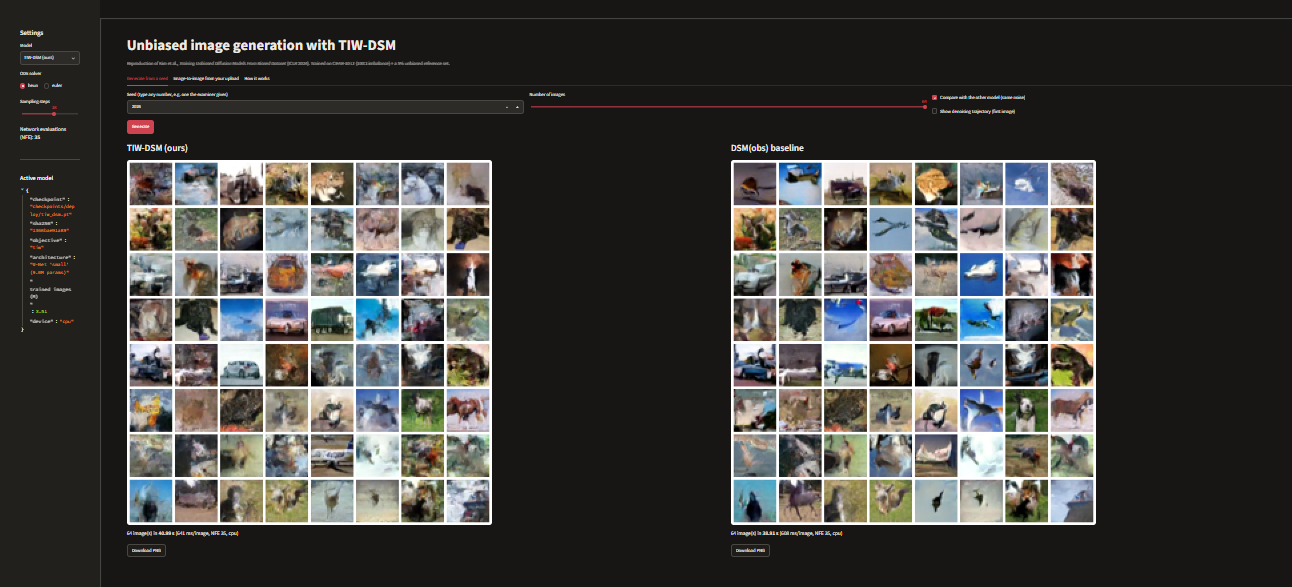
\includegraphics[width=\linewidth,trim={192.9mm 16.7mm 51.3mm 42.3mm},clip]{figures/app_compare64.png}\\[-1pt]
\small DSM(obs)
\end{minipage}\hfill
\begin{minipage}{.48\linewidth}\centering
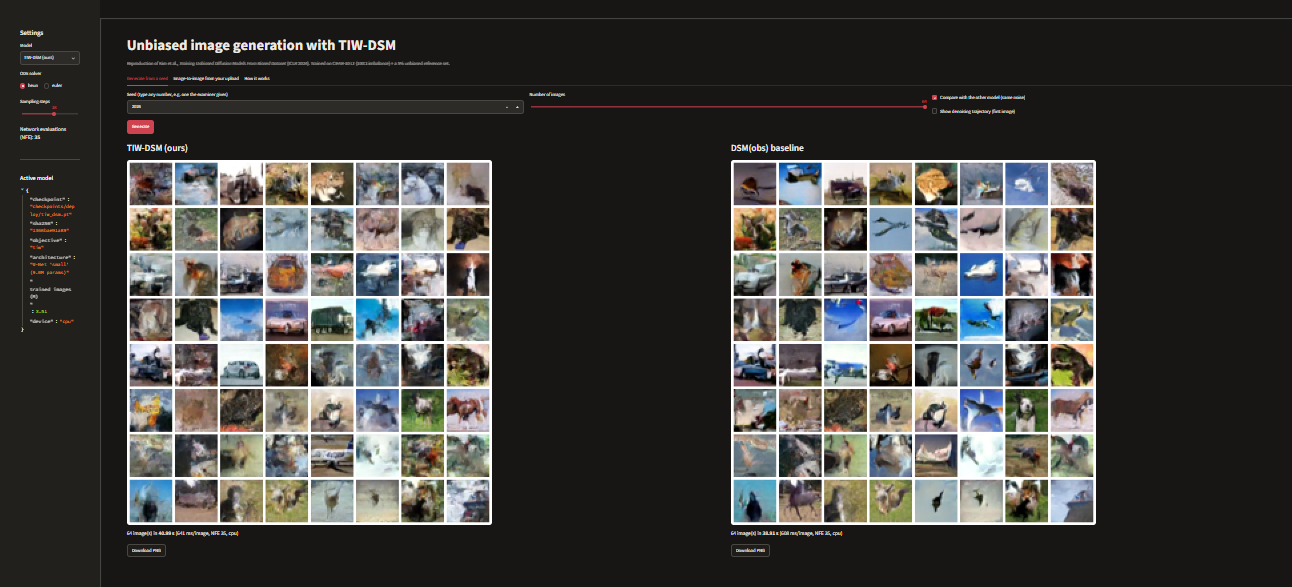
\includegraphics[width=\linewidth,trim={33.3mm 16.7mm 211.2mm 42.3mm},clip]{figures/app_compare64.png}\\[-1pt]
\small TIW DSM
\end{minipage}
\caption[Paired samples from the application]{The two grids come from the same hosted comparison: 64 images per model, starting seed 2026, Heun sampler and 35 network evaluations. Corresponding grid positions start from the same noise. This controls the inference input, not the randomness of training.}\label{fig:samples}
\end{figure}
Some objects are recognisable and others are difficult to identify. The grids let a reader see that ambiguity for the same inputs. The evidence for a change in class balance comes from the full evaluation, not from selecting particular images in this figure.


\clearpage
\section{Additional experiment: sampling cost, quality and balance}\label{sec:extra}
\subsection{Question and expectations}
A user waiting for an image can change the sampler without retraining the model. We therefore asked how many denoiser calls were worth making and whether a faster setting would preserve the change in class balance. The paper uses 35 calls for its main experiment. Our study varied the solver and the number of calls while keeping the model weights fixed. This is a separate inference experiment, not simply a shorter training run.

We tested three expectations. First, we expected FID to improve rapidly up to about 20 to 35 network evaluations and then change little. At the same number of calls, we expected second order Heun to outperform first order Euler. Second, if the learned score determined most of the class balance, TIW should retain lower bias at every budget. Third, inference time should grow roughly in proportion to the number of calls, with no extra discriminator cost for TIW.

\subsection{Controlled comparison}
We used the same two EMA checkpoints as in Table~\ref{tab:main}. For $N$ steps, Heun uses $2N-1$ denoiser calls here and Euler uses $N$. We tested Heun at 3, 5, 9, 13, 18 and 25 steps, pairing these with Euler at 5, 9, 17, 25, 35 and 49 steps. The resulting 24 combinations cover two models, two solvers and six matched call budgets. Every combination used the same noise seeds and produced \resStepsN{} images.

We compared FID, recall, Equation 51 bias and tail share, together with time per image in batches of 500 and the time to generate one image. The latter is the median of five measurements after an initial warm up on a \resStepsDevice{}. Precision and recall were part of the wider evaluation; the archived comparison by solver reports recall. The FID estimates in this section are comparable \emph{within} the study. They should not be read as changes from Table~\ref{tab:main}, which uses 50,000 generated images rather than 10,000.
\begin{figure}[H]\centering
\asset[width=\linewidth]{steps_experiment.png}
\caption[Effects of the sampling budget]{FID, recall, bias and generation time as the number of denoiser calls increases. Solid lines represent Heun, dotted lines represent Euler, and colour identifies the model.}\label{fig:steps}
\end{figure}
\begin{table}[H]\centering
\caption[All sampling configurations]{All 24 settings, using \resStepsN{} generated images each. The last two columns give milliseconds per image in a batch of 500 and milliseconds for a single image.}\label{tab:steps}
\footnotesize\setlength{\tabcolsep}{4pt}
\begin{tabular}{llrrrrrrrr}\toprule
Model & Solver & Steps & Calls & FID & Recall & Bias & Tail (\%) & Batch (ms) & Single (ms)\\\midrule
\rowsfile{steps_rows}
\bottomrule\end{tabular}\end{table}

\subsection{Where more computation helped}
\lead{Quality.} At the default of 18 Heun steps, FID was \resStepsFIDrefobs{} for DSM(obs) and \resStepsFIDreftiw{} for TIW. The baseline gained little from extending Heun beyond 25 calls: its FID was 41.96 at 17 calls, 37.76 at 25, 37.44 at 35 and 37.55 at 49. At just five calls, Heun gave FID near 339 for both models; Euler was near 90. Our first expectation was therefore only partly supported. Heun beat Euler for the baseline at the tested budgets of 17 calls and above, but not for TIW. For TIW, Euler gave FID 55.40 against 68.47 at 17 calls, and 52.16 against 53.13 at 35. Euler also had higher recall for TIW across the tested budgets.

\lead{Class balance.} At the default, bias was \resStepsBiasrefobs{} for DSM(obs) and \resStepsBiasreftiw{} for TIW. For both solvers, TIW had lower bias than the baseline at every tested budget from 17 calls upward. We cannot extend that conclusion to every budget: at five or nine calls, poor images make the classifier difficult to interpret. The solver also matters. From 17 to 49 calls, Euler gave TIW a tail share between 41.8\% and 47.0\%; the corresponding Heun shares lay between 50.2\% and 56.3\%. The trained weights alone did not determine the final class mix.

\lead{Time.} On the T4, each additional call cost approximately 1.3 milliseconds per image in a batch and about 15 milliseconds when generating a single image. The two models use the same denoiser architecture and number of calls. Measured times differ slightly, but the application does not need a discriminator pass at inference.

\lead{Choice for the demonstration.} Among the Heun settings, the cheapest TIW result within 10\% of the best Heun FID used 13 steps, or \resStepsKneeNFE{} calls. Its FID of \resStepsKneeFID{} was about 8.5\% above the best Heun result of 51.90. It used about 71\% as many calls as the default and gave bias 0.370. Across \emph{both} solvers, Euler at 17 calls was the cheapest setting within 10\% of the overall best FID (55.40 against 51.64), but its bias was higher at 0.420. The deployed interface offers Heun at 13 steps as an option. Its default remains Heun at 18 steps, or 35 calls, and its list of step counts does not include 17.

\section{Analysis and discussion}\label{sec:discussion}
\subsection{What improved, and what did not?}
TIW reduced our measured class bias, but its gains were uneven. Automobiles fell from 15.1\% to 6.7\%, while ships reached 11.0\%. Trucks at 17.0\% and deer at 14.5\% exceeded the 10\% target. Birds at 4.1\% and dogs at 4.3\% remained uncommon. Deer and birds are not among the five classes we defined as the tail. The ratio between the largest and smallest generated class shares improved from about 7.6 to 4.2, still far from one.

Our FID increased by 16.10 points where the paper reported an improvement of 1.48 points. Recall also fell. The fair conclusion is that class balance improved \emph{in this run}, not that a loss of diversity is an inevitable cost of correcting bias. Likewise, better precision here does not undo the weaker recall or FID.

\subsection{What the source probabilities can tell us}
On the training images in Table~\ref{tab:disc}, balanced accuracy was about 99\% for $\tau\leq0.1$, 94.8\% at 0.3, 70.5\% at 0.5 and 50\% at 1.0. The mean probabilities approach 0.5 as noise increases, consistent with mixture weights moving towards one. This is the qualitative behaviour the paper predicts. It is not a measurement of ratio calibration or of the size of the input gradient.

At low noise, median raw odds for biased images were between about $10^{-7}$ and $10^{-5}$. Many such examples may therefore have received very little weight. One plausible explanation for lower recall is that the small reference set had too much influence. There is a useful limit to this explanation: below a raw probability of $10^{-5}$, our stored training weight has a floor of $2\times10^{-5}$ and the derivative through the clamp is zero. The diagnostics do not show that these examples received a large correction, nor that \emph{every} biased example was suppressed. We did not measure ratio error on independent images, effective sample size by source, or the effect of stopping the discriminator earlier. Overfitting is a hypothesis, not an established cause of the FID result.

\subsection{Other explanations we could not separate}
The denoising network had \resParams{} million parameters rather than approximately 56 million. Both methods used the smaller network, but limited capacity need not affect them equally. We also used flips rather than the full EDM augmentation policy (probability 0.12) on only 10,380 distinct images. This may increase memorisation; we did not test it directly.

At our matched checkpoint the learning rate had reached only about 35\% of its peak. Longer training helped DSM(obs) substantially, but we have no corresponding TIW measurement at 11 million exposures. Clipped probabilities, gradient safeguards, automatic mixed precision and the ADM compatibility edit are further differences. Their individual effects are unknown. The two FID implementations use the same family of Inception weights, but preprocessing and numerical routines can still differ; we did not run both evaluators on identical samples. Finally, both the paper and our reproduction use a reference set of 500 images in this setting. Its small size and classifier errors complicate the measurement, but the reference size itself is not a deviation from the original study.

\subsection{What the toy and sampling experiments add}
In the two dimensional example, the minority share under weighting alone (\resToytiwW{}) stayed close to ordinary DSM (\resToyobs{}). This agrees with the conditional mean argument in Section~\ref{sec:whyboth} and with the authors' comparison of FID 13.27 using weighting alone against 12.99 without it. With an exact ratio, it is the correction that changes the target score. Weighting changes where training effort goes. The clean image estimator is different: very uneven clean weights can leave a few examples dominating the gradient and reduce effective sample size. This offers an explanation for, but does not by itself prove the cause of, the paper's IW result of 15.79 against 12.99 for DSM(obs).

The sampling study addresses a practical decision that training comparisons do not answer. One can reduce waiting time without fitting new weights, but the faster solver need not preserve the same balance. For this model, choosing between Euler at 17 calls and Heun at 25 calls means deciding whether the lower cost or the closer class distribution matters more.

\section{Model deployment}\label{sec:deploy}
\subsection{From a seed or photograph to an output image}
\begin{figure}[H]\centering
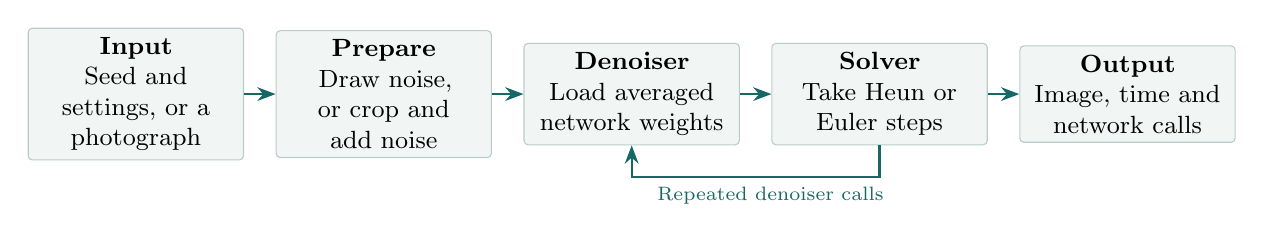
\begin{tikzpicture}[node distance=4mm,box/.style={draw=Rule,fill=Pale,rounded corners=1.5pt,align=center,font=\small,minimum height=12mm,text width=25mm},arr/.style={-{Stealth},thick,Accent}]
\node[box] (in) {\textbf{Input}\\Seed and settings, or a photograph};
\node[box,right=of in] (prep) {\textbf{Prepare}\\Draw noise, or crop and add noise};
\node[box,right=of prep] (net) {\textbf{Denoiser}\\Load averaged network weights};
\node[box,right=of net] (solver) {\textbf{Solver}\\Take Heun or Euler steps};
\node[box,right=of solver] (out) {\textbf{Output}\\Image, time and network calls};
\draw[arr] (in) -- (prep);\draw[arr] (prep) -- (net);\draw[arr] (net) -- (solver);\draw[arr] (solver) -- (out);
\draw[arr] (solver.south) -- ++(0,-4mm) -| node[pos=.22,below,font=\scriptsize]{Repeated denoiser calls} (net.south);
\end{tikzpicture}
\caption[How inference works]{Only the denoiser and solver are needed to generate images. A separately installed classifier can label outputs in a local installation; it is not part of the hosted inference path.}\label{fig:pipeline}
\end{figure}
On the \textit{Generate} tab, the user chooses a seed, image count, solver and step count. The seed fixes the initial noise, not an object class. Selecting both models pairs their starting noise. Uploading a photograph starts a different procedure automatically: the application takes a centre crop, resizes it to $32\times32$, adds noise and solves the denoising ordinary differential equation. This editing procedure follows the idea behind SDEdit \cite{meng2022sdedit}.

The information tab explains the process; the sidebar identifies the checkpoint, objective, model size, training exposure and device. A new seed or upload exercises the model directly. A screenshot documents only the run shown.

\subsection{Hosting and local startup}
The demonstration runs on a CPU on Streamlit Community Cloud at \appURL{}. Both model files are in the repository, and \texttt{app/requirements.txt} lists the hosted dependencies. Class predictions and histograms are available only locally with \texttt{checkpoints/eval\_classifier\_vgg13bn.ts}.

With compatible versions of Python and PyTorch, run these commands from the repository root. Generation needs neither a dataset download nor a CUDA device.
\begin{lstlisting}
python -m pip install -r requirements.txt
python -m streamlit run app/streamlit_app.py
\end{lstlisting}
Open \url{http://localhost:8501}. For the published comparison, use the released weights rather than final snapshots from runs of different lengths.

\subsection{Running the model from Python}
This CPU example returns 16 images as an array of unsigned bytes with shape $(16,32,32,3)$.
\par\noindent\begin{minipage}{\linewidth}
\begin{lstlisting}[language=Python]
from tiwdsm.io import load_ema
from tiwdsm.edm import sample, seeded_latents
from tiwdsm.data import to_uint8

model, meta = load_ema("checkpoints/deploy/tiw_dsm.pt", "cpu")
z = seeded_latents(range(2026, 2026 + 16), "cpu")
imgs = to_uint8(sample(model, z, num_steps=18, solver="heun"))
\end{lstlisting}
\end{minipage}\par
During the main TIW evaluation on a Kaggle T4, inference at 35 calls took \resMsImg{} milliseconds per image in batches of 500. The separate solver experiment measured about 0.53 seconds for one image at that budget. These measurements are distinct from the elapsed times displayed in the browser.

\subsection{Application inputs and outputs}
\begin{table}[H]\centering
\caption[Application inputs and outputs]{Accepted inputs, transformations and outputs of the deployment.}\label{tab:io}
\small\begin{tabularx}{\linewidth}{@{}P{32mm}Y@{}}\toprule
Item & Detail\\\midrule
Generation & Integer seed $0\leq s<2^{31}$; 1, 4, 8, 16, 32 or 64 images; Heun or Euler; 3, 5, 9, 13, 18, 25, 35 or 49 steps; TIW or DSM(obs).\\
Upload & PNG, JPEG, WebP or BMP of any size; starting noise strength $0.2\leq\sigma\leq20$ and a noise seed.\\
Input preparation & Image $k$ uses \texttt{torch.Generator().manual\_seed(seed+k)}. Standard Gaussian noise is scaled by $\sigma_{\max}=80$. For an upload, crop to a square, resize with bicubic interpolation, apply $x/127.5-1$ and add $\sigma$ times standard Gaussian noise.\\
Model output & A floating point tensor with shape $[n,3,32,32]$. Clamp its entries to $[-1,1]$ and convert to unsigned bytes with shape $[n,32,32,3]$.\\
Hosted display & A grid and downloadable PNG, elapsed time, milliseconds per image, call count and optional denoising trajectory. The upload view shows the input, the noisy input and the model output, with trajectory support.\\
Local option & Class predictions, confidence and a histogram when the VGG13 helper is present.\\\bottomrule
\end{tabularx}\end{table}

\subsection{What the live tests showed}
\begin{figure}[H]\centering
\asset[width=.94\linewidth]{app_generate.png}
\caption[Generating images from a seed]{With seed 2026, the hosted application generated 16 images per model using 18 Heun steps and 35 calls. The CPU display shows 9.88 seconds for TIW and 8.94 seconds for DSM(obs). The first image's denoising trajectory and the TIW checkpoint prefix \texttt{1366bae91a89} are visible. The sidebar reports objective \texttt{tiw} and 3.51 million training exposures.}\label{fig:app1}
\end{figure}
\begin{figure}[H]\centering
\asset[width=\linewidth]{app_upload.png}
\caption[Editing a photograph of a cat]{The input file was \texttt{cat.jpg}. From left: the crop at $32\times32$, the same crop after adding noise at $\sigma=0.5$, and the model output. With noise seed 0 and 13 Heun steps (25 calls), the hosted CPU displayed 0.92 seconds.}\label{fig:app2}
\end{figure}
The cat remained recognisable in outline, but the output was blurred and facial details changed. This test shows that the application could decode, resize, perturb and process a new photograph. It does not show that the edited image is more faithful than the input. We did not measure peak signal to noise ratio, structural similarity or any perceptual restoration score.
\begin{figure}[H]\centering
\asset[width=.96\linewidth]{app_incognito.png}
\caption[Generation in an Incognito session]{With the Incognito indicator visible, seed 1234 produced one image per model using 18 Heun steps and 35 calls. The hosted CPU displayed 2.39 seconds for TIW and 1.90 seconds for DSM(obs). This records one successful browser session, not a general timing benchmark or an audit of public access.}\label{fig:incognito}
\end{figure}


\section{Limitations}\label{sec:limits}
\lead{Scale and experimental control.} We matched the image data, denoiser architecture, effective batch size, number of training exposures and main evaluation protocol. Our network was smaller than the paper's, augmentation was limited to flips and the matched comparison ended during the learning rate ramp. TIW accumulated smaller batches and took a different path through the training code. Equal nominal seeds are therefore not a guarantee of identical initialisation or noise. We can describe a difference between these runs, but cannot assign all of it to the loss function.

\lead{Training variation.} Each image model was trained once. We used one discriminator trained for 10,000 updates and did not compare it with an earlier or less confident version. The three seeds used in the toy experiment are not three independent image training runs. We have neither a measure of variation between image training runs nor a calibration test on held out images. Clipping, gradient handling and mixed precision also separate the implemented loss from the exact theoretical objective.

\lead{Scope of the reproduction.} We studied only the long tailed CIFAR 10 experiment with a 5\% reference set. We did not reproduce CIFAR 100, FFHQ, CelebA or the other reference sizes. DSM(obs) was the only baseline trained on images alongside TIW. The reference only model, clean importance weighting and variants without weighting or correction were implemented and tested in two dimensions only. The code exposes these through \texttt{--mode iw}, \texttt{--mode ref}, \texttt{--no\_reweight} and \texttt{--no\_correction}.

\lead{Meaning of bias.} The reference set defines the target; the method cannot decide whether that target is fair. With 500 images and a largest to smallest class ratio of 1.625, the reference itself has sampling variation. The VGG13 evaluator was trained on real images, and we did not correct its errors on generated examples. Our measures describe the frequencies of ten classes, not every visual or social form of bias. The 120 images shared between the sources were retained for fidelity to the released experiment, and their effect was not measured separately.

\lead{Archive and demonstration.} The published checkpoints, figures and numerical summaries allow others to inspect and evaluate the trained models. They do not include every raw training log or an exact record of all software versions. Evaluating saved weights is different from reproducing their training. The application generates at $32\times32$ resolution; its screenshots demonstrate specific runs rather than general robustness, restoration quality or freedom from bias. Optional local class labels are not part of the hosted demonstration.

\section{Conclusion}\label{sec:conclusion}
The original question was whether a small reference collection could teach a diffusion model what to generate more or less often. With the authors' 10,000 biased images and 500 reference images, we found evidence that it could. At equal training exposure the five rare classes accounted for \resTailtiw\% of TIW output, compared with \resTailobs\% for the baseline. The reference based bias score fell by \resBiasRed\%. The individual classes did not all reach their target of 10\%.

Our implementation used the mixture weight $2d$ and the correction $\sigma^2\nabla\log d$, with the clipping and numerical safeguards documented in Section~\ref{sec:practical}. The two dimensional test helped distinguish the role of the correction from that of the weight. On images, TIW obtained FID \resFIDtiw{} against \resFIDobs{} for ordinary DSM, with lower recall. This is a partial reproduction: the balance result improved, but the original paper's improvement in FID did not carry over. Extreme discriminator predictions are one possible explanation, not a demonstrated cause.

For the two trained models, TIW retained lower measured bias with either solver at all tested budgets of 17 calls or more. Heun at 13 steps is a reasonable option when waiting time matters. The deployed default remains 18 Heun steps. Generation from a seed, the cat upload and the Incognito test demonstrate how the saved model behaves outside the training notebook; none replaces evaluation on a large sample.

The most useful next experiment would test the discriminator on images it did not see during training. Measuring calibration, effective weight and correction size separately by source, then varying early stopping, regularisation and the numerical safeguards, would help distinguish competing explanations. Longer matched runs, more seeds, a larger network, the original augmentation and tests of each loss term on images would show which results persist.

\clearpage
\section{References}\label{sec:refs}
\begingroup
\small
\renewcommand{\section}[2]{}
\let\originalbibliography\thebibliography
\renewcommand{\thebibliography}[1]{\originalbibliography{#1}\setlength{\itemsep}{1.3pt}\setlength{\parsep}{0pt}}
\bibliographystyle{ieeetr}
\bibliography{references}
\endgroup
\appendix

\section{Changes since the mid evaluation report}\label{app:revisions}
The review now connects density ratio estimation \cite{sugiyama2012dre}, EDM, discriminator guidance and the ADM encoder. We derive the mixture weight $2d$ from Equation 36 of the paper, give the denoiser form in Equation~\ref{eq:edmtiw} and explain why weighting alone leaves the conditional DSM target unchanged.

The exact reference class ratio is $65/40=1.625$; the mid evaluation notebook displayed 1.62 and the report displayed 1.63. We clarify why the recovered class labels are for analysis only and describe reference repetition and noise perturbation in the training pipeline.

We added the Equation 51 bias measure, identified the VGG13 classifier and included generative recall \cite{kynkaanniemi2019pr}. The proposal and mid report used \emph{35 steps} loosely. Here, 18 Heun steps require 35 network evaluations. The solver study reports both counts.

\section{Reproducing the reported runs}\label{app:commands}
\subsection{Identify the code and weights}
We inspected commit \texttt{ef6dae43fd7bdae7387b70a45eea891972b6e8e7}, dated 24 November 2026 \cite{team2026repro}. Its PDF was identical in bytes to the team's report before correction. This edition revises the writing; the checkpoints, measurements and figures are unchanged.

Both deployment files correspond to \texttt{ema\_003512k.pt}, saved at 3,512,320 exposures. The SHA 256 prefixes agree with those in \texttt{results/eval\_obs.json} and \texttt{results/eval\_tiw.json}. The complete file identifiers are:
\begin{lstlisting}
checkpoints/deploy/dsm_obs.pt
ab1183b3a4eac00aac3f88a9b7ec4ef5a0f6f38799b40f6cc8ec5a29948512f2

checkpoints/deploy/tiw_dsm.pt
1366bae91a890407772bfabeae1f452e72304d5fc06e8c2dca49811c466a543c
\end{lstlisting}

\subsection{Evaluate the released checkpoints}
From the project root, prepare the research data and evaluation models, including Inception and VGG13. Full evaluation on a CPU is expensive. New output names protect the archived results. The backslashes below continue shell commands onto another line. In PowerShell, omit them and enter each command on one line.
\par\noindent\begin{minipage}{\linewidth}
\begin{lstlisting}
python -m pip install -r requirements.txt
python scripts/prepare_data.py
python scripts/evaluate.py --ckpt checkpoints/deploy/dsm_obs.pt \
  --name reeval_obs --num 50000 --steps 18 --solver heun --batch 500 \
  --seed_offset 0
python scripts/evaluate.py --ckpt checkpoints/deploy/tiw_dsm.pt \
  --name reeval_tiw --num 50000 --steps 18 --solver heun --batch 500 \
  --seed_offset 0
python scripts/evaluate.py --real bias --name reeval_data_bias
python scripts/evaluate.py --real ref --name reeval_data_ref
python scripts/evaluate.py --real target --name reeval_data_target
python scripts/steps_experiment.py --ckpt obs=checkpoints/deploy/dsm_obs.pt \
  --ckpt tiw=checkpoints/deploy/tiw_dsm.pt --num 10000 --batch 500 \
  --out results/steps_reeval.json
\end{lstlisting}
\end{minipage}\par
Use a fresh solver results path: the script checks the model label, solver and step count but not the checkpoint identity when it skips completed settings. Hardware and libraries can change measurements. A replacement classifier changes the evaluation configuration. The baseline at 11 million exposures needs a separate checkpoint not included with the two deployment files.

\subsection{Train two models at the same exposure budget}
The historical baseline reached 11 million exposures and TIW reached 3.91 million. For the main comparison we evaluated their earlier, shared checkpoint. The commands below instead request new training runs with the same final budget of 3.51232 million exposures. Use new output directories. One CUDA processor can run them sequentially; the original runs used separate T4 processors in parallel.
\par\noindent\begin{minipage}{\linewidth}
\begin{lstlisting}
python scripts/toy_2d.py
python scripts/train_discriminator.py --iters 10000 --batch 128 \
  --lr 0.0003 --seed 0 --backbone adm --out checkpoints/recheck_discriminator.pt
python scripts/train_score.py --mode obs --outdir runs/recheck_obs \
  --preset small --batch 256 --accum 1 --lr 0.001 --lr_rampup_kimg 10000 \
  --ema_halflife_kimg 500 --duration_mimg 3.51232 --snapshot_kimg 500 \
  --time_limit_h 11.3 --seed 0 --amp
python scripts/train_score.py --mode tiw --outdir runs/recheck_tiw \
  --disc checkpoints/recheck_discriminator.pt --preset small --batch 256 \
  --accum 2 --lr 0.001 --lr_rampup_kimg 10000 --ema_halflife_kimg 500 \
  --duration_mimg 3.51232 --snapshot_kimg 500 --time_limit_h 11.3 --seed 0 --amp
\end{lstlisting}
\end{minipage}\par
When both runs finish, evaluate each new \texttt{ema\_003512k.pt} rather than final snapshots of different lengths. A run interrupted by its time limit can be resumed with the same command. Not every state of the random number generators used by the device and data loader is saved, so resumption need not be identical in every bit. Record results of new evaluations as new measurements. Repeated training runs would be needed to estimate variability.

\subsection{Compile the report or start the application}
The LaTeX project includes the measured tables, bibliography and figures. Compiling the report does not require training, downloading data or regenerating figures.
\begin{lstlisting}
# From the folder containing main.tex:
latexmk -pdf -interaction=nonstopmode -halt-on-error main.tex

# Alternatively, in that same folder:
pdflatex main.tex
bibtex main
pdflatex main.tex
pdflatex main.tex

# From the project repository root:
python -m streamlit run app/streamlit_app.py
\end{lstlisting}
The optional script that regenerates the report figures needs the original raw training logs to draw the learning curves. Without those logs it can overwrite existing results with missing values. Use the supplied figures for this report. Rebuild them only when documenting a new experiment with its own complete records.
\end{document}
